%%%%%%%%%%%%%%%%%%%%%%%%%%%%%%%%%%%%%%%%%
% Beamer Presentation
% LaTeX Template
% Version 1.0 (10/11/12)
%
% This template has been downloaded from:
% http://www.LaTeXTemplates.com
%
% License:
% CC BY-NC-SA 3.0 (http://creativecommons.org/licenses/by-nc-sa/3.0/)
%
%%%%%%%%%%%%%%%%%%%%%%%%%%%%%%%%%%%%%%%%%

%----------------------------------------------------------------------------------------
%	PACKAGES AND THEMES
%----------------------------------------------------------------------------------------

\documentclass{beamer}

\usepackage{helvet}
\renewcommand{\familydefault}{\sfdefault}

\usepackage{inconsolata}
%\usepackage[T1]{fontenc}
%\usepackage{libertine}
\usepackage{listings}
\lstset{language=C++,
  basicstyle=\tiny\ttfamily,
  keywordstyle=\tiny\color{blue}\ttfamily
}

% use Unicode characters - try changing the option if you run into troubles with special characters (e.g. umlauts)
\usepackage[utf8]{inputenc}

% clean citations
\usepackage{cite}

% hyperref makes references clicky. use \url{www.example.com} or \href{www.example.com}{description} to add a clicky url
\usepackage{nameref,hyperref}

\usepackage[export]{adjustbox}


\mode<presentation> {

% The Beamer class comes with a number of default slide themes
% which change the colors and layouts of slides. Below this is a list
% of all the themes, uncomment each in turn to see what they look like.

%\usetheme{default}
%\usetheme{AnnArbor}
\usetheme{Antibes}
%\usetheme{Bergen}
%\usetheme{Berkeley}
%\usetheme{Berlin}
%\usetheme{Boadilla}
%\usetheme{CambridgeUS}
%\usetheme{Copenhagen}
%\usetheme{Darmstadt}
%\usetheme{Dresden}
%\usetheme{Frankfurt}
%\usetheme{Goettingen}
%\usetheme{Hannover}
%\usetheme{Ilmenau}
%\usetheme{JuanLesPins}
%\usetheme{Luebeck}
%\usetheme{Madrid}
%\usetheme{Malmoe}
%\usetheme{Marburg}
%\usetheme{Montpellier}
%\usetheme{PaloAlto}
%\usetheme{Pittsburgh}
%\usetheme{Rochester}
%\usetheme{Singapore}
%\usetheme{Szeged}
%\usetheme{Warsaw}

% As well as themes, the Beamer class has a number of color themes
% for any slide theme. Uncomment each of these in turn to see how it
% changes the colors of your current slide theme.

%\usecolortheme{albatross}
%\usecolortheme{beaver}
%\usecolortheme{beetle}
%\usecolortheme{crane}
%\usecolortheme{dolphin}
%\usecolortheme{dove}
%\usecolortheme{fly}
%\usecolortheme{lily}
%\usecolortheme{orchid}
%\usecolortheme{rose}
%\usecolortheme{seagull}
%\usecolortheme{seahorse}
%\usecolortheme{whale}
%\usecolortheme{wolverine}

%\setbeamertemplate{footline} % To remove the footer line in all slides uncomment this line
%\setbeamertemplate{footline}[page number] % To replace the footer line in all slides with a simple slide count uncomment this line

%\setbeamertemplate{navigation symbols}{} % To remove the navigation symbols from the bottom of all slides uncomment this line

\setbeamertemplate{navigation symbols}{}
}



\usepackage{graphicx} % Allows including images
\usepackage{booktabs} % Allows the use of \toprule, \midrule and \bottomrule in tables
\usepackage{comment}

%----------------------------------------------------------------------------------------
%	TITLE PAGE
%----------------------------------------------------------------------------------------

\title[\textsc{dsgvg} @ LAW\&LSD]{Dynamic succinct genome variation graphs} % The short title appears at the bottom of every slide, the full title is only on the title page

\author{Erik Garrison} % Your name
\institute[UCSC] % Your institution as it will appear on the bottom of every slide, may be shorthand to save space
{
University of California, Santa Cruz \\ % Your institution for the title page
\medskip
\textit{erik.garrison@gmail.com} % Your email address
}
\date{\today} % Date, can be changed to a custom date

\begin{document}

\begin{frame}
\titlepage % Print the title page as the first slide
\end{frame}

\begin{frame}
\frametitle{Overview} % Table of contents slide, comment this block out to remove it
\tableofcontents % Throughout your presentation, if you choose to use \section{} and \subsection{} commands, these will automatically be printed on this slide as an overview of your presentation
\end{frame}

%----------------------------------------------------------------------------------------
%	PRESENTATION SLIDES
%----------------------------------------------------------------------------------------

%------------------------------------------------
\section{Variation graphs} % Sections can be created in order to organize your presentation into discrete blocks, all sections and subsections are automatically printed in the table of contents as an overview of the talk
%------------------------------------------------

\subsection{Motivation}

\begin{frame}
  \frametitle{Biological understanding via sequence comparison}
In biology, we are interested in understanding the mutual relations in collections of biosequences (DNA, RNA, and proteins).

\begin{figure}
  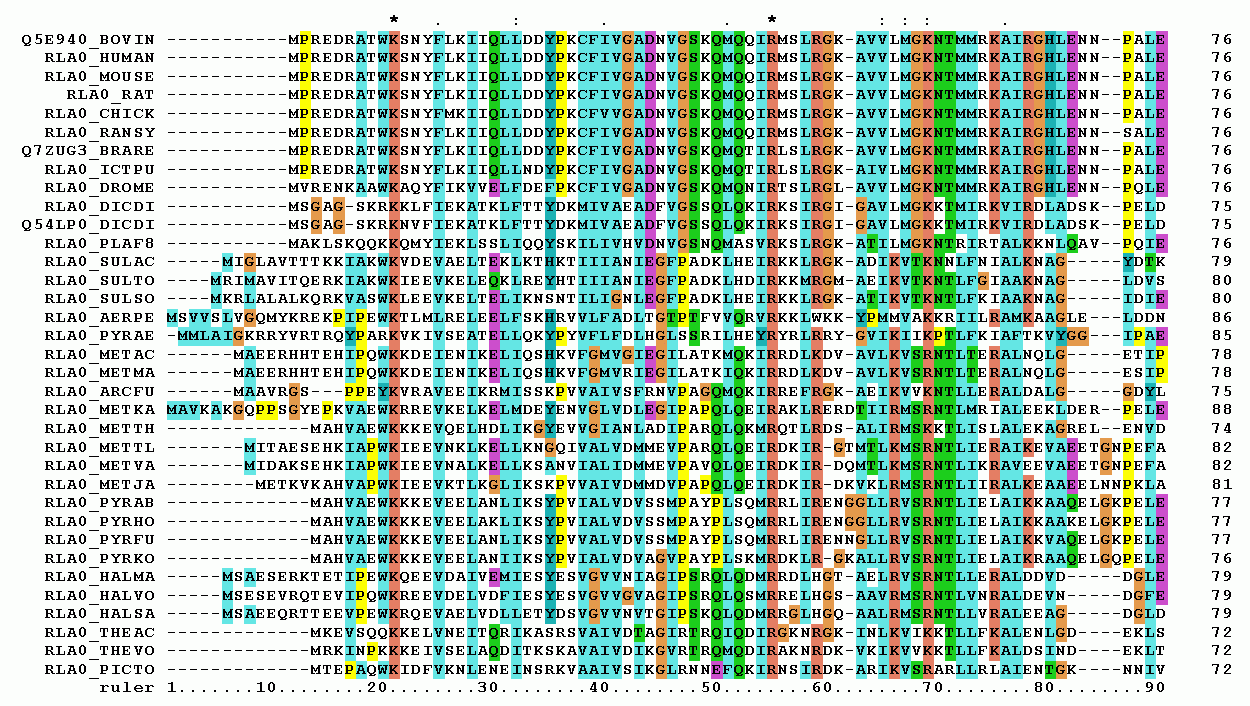
\includegraphics[scale=0.2,center]{RPLP0_90_ClustalW_aln.png}
\end{figure}


\end{frame}

\begin{frame}
    \frametitle{Resequencing}
With large genomes, we have tended to do this via linear reference models.

\begin{figure}
  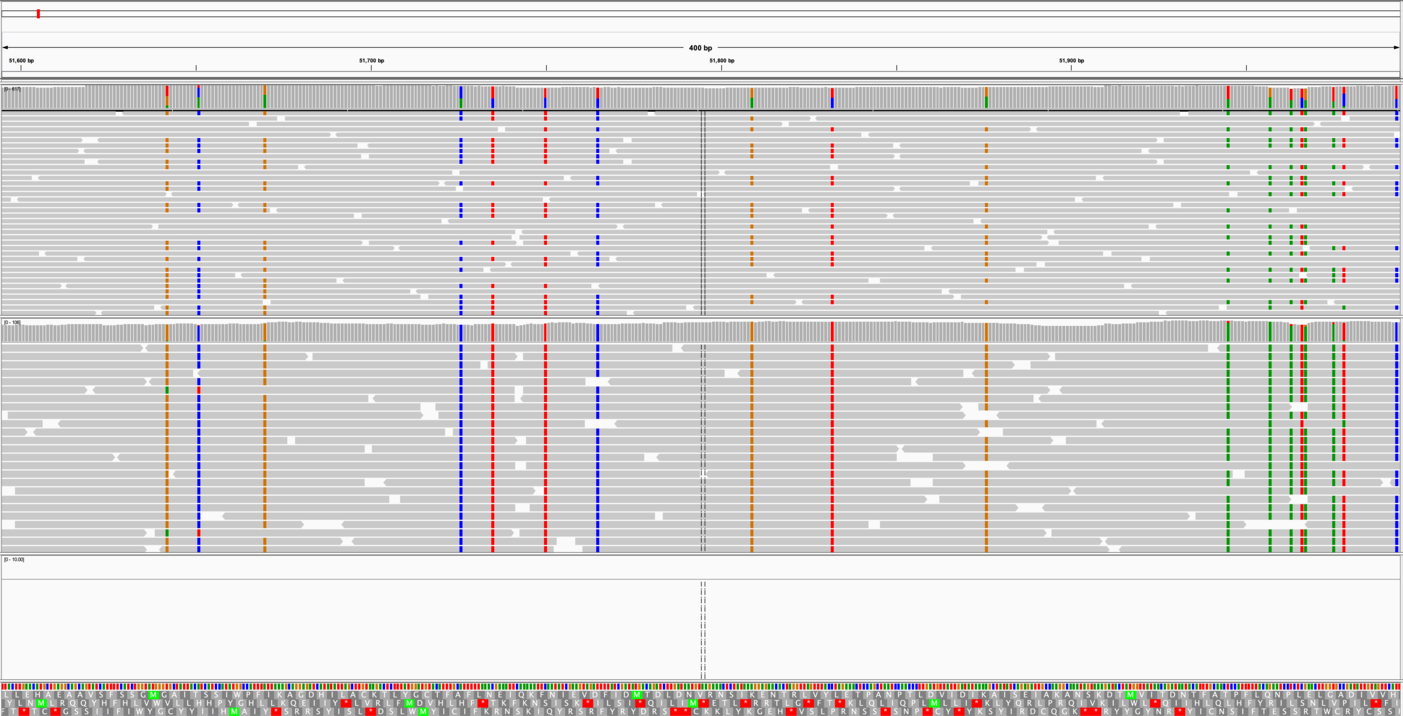
\includegraphics[scale=0.2,center]{TqkY9nw1.png}
\end{figure}
\end{frame}

\begin{frame}
  \frametitle{Reference bias}
  But this can introduce bias.
%  \\~\\
%  The more different an allele is from the reference, the more difficult it is to describe accurately in terms of this reference.

  \begin{figure}
    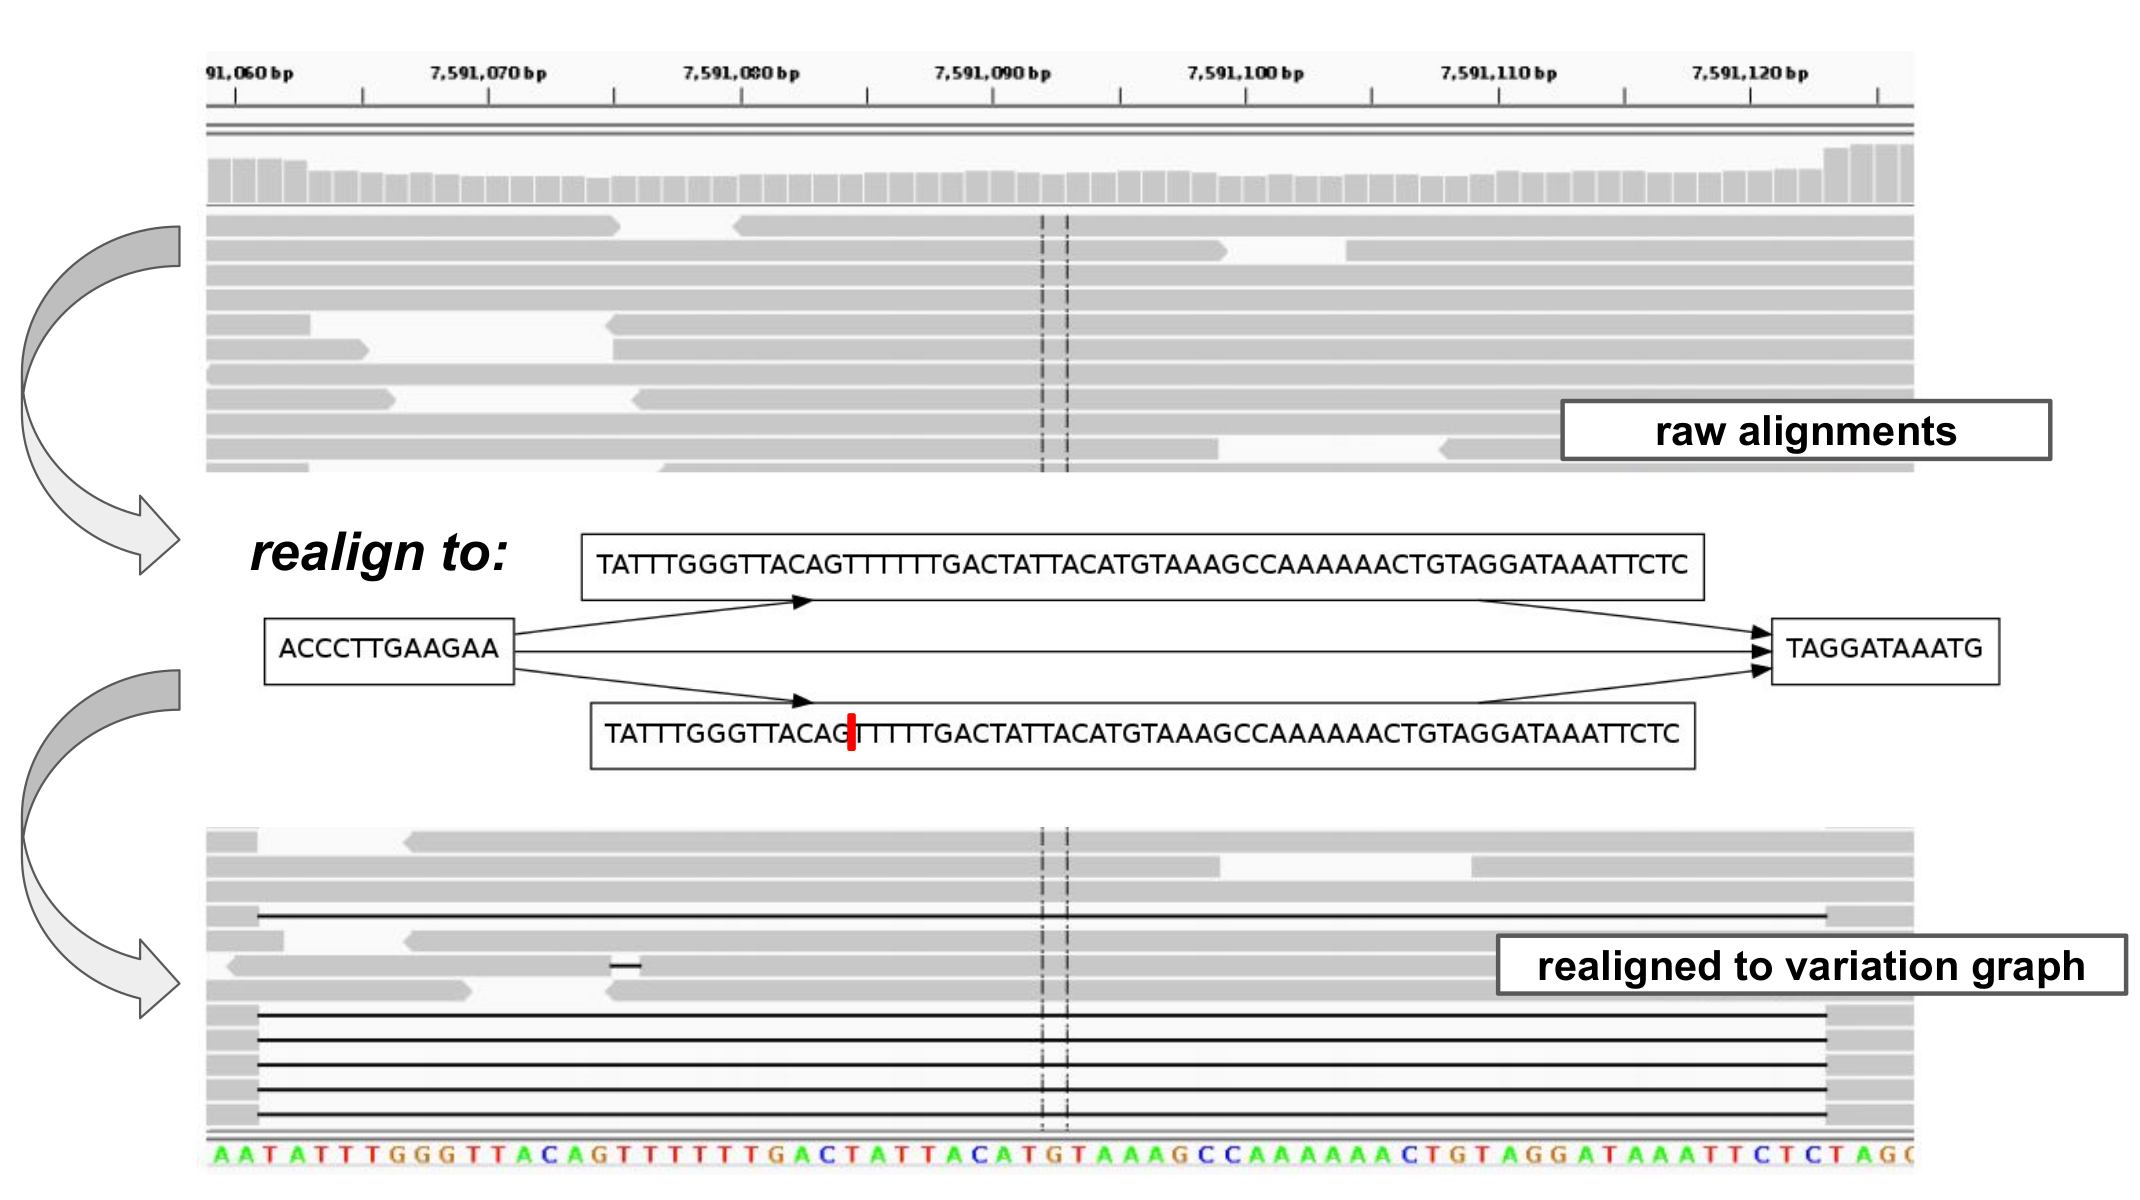
\includegraphics[scale=0.14,center]{igv_graph_realign.png}
    \end{figure}
\end{frame}


\begin{frame}
    \frametitle{Archival ``variant graphs'' project texts into a graph}
%Textual ``variant graphs'' allow the compact description of a set of versions of a text.

    \begin{figure}
      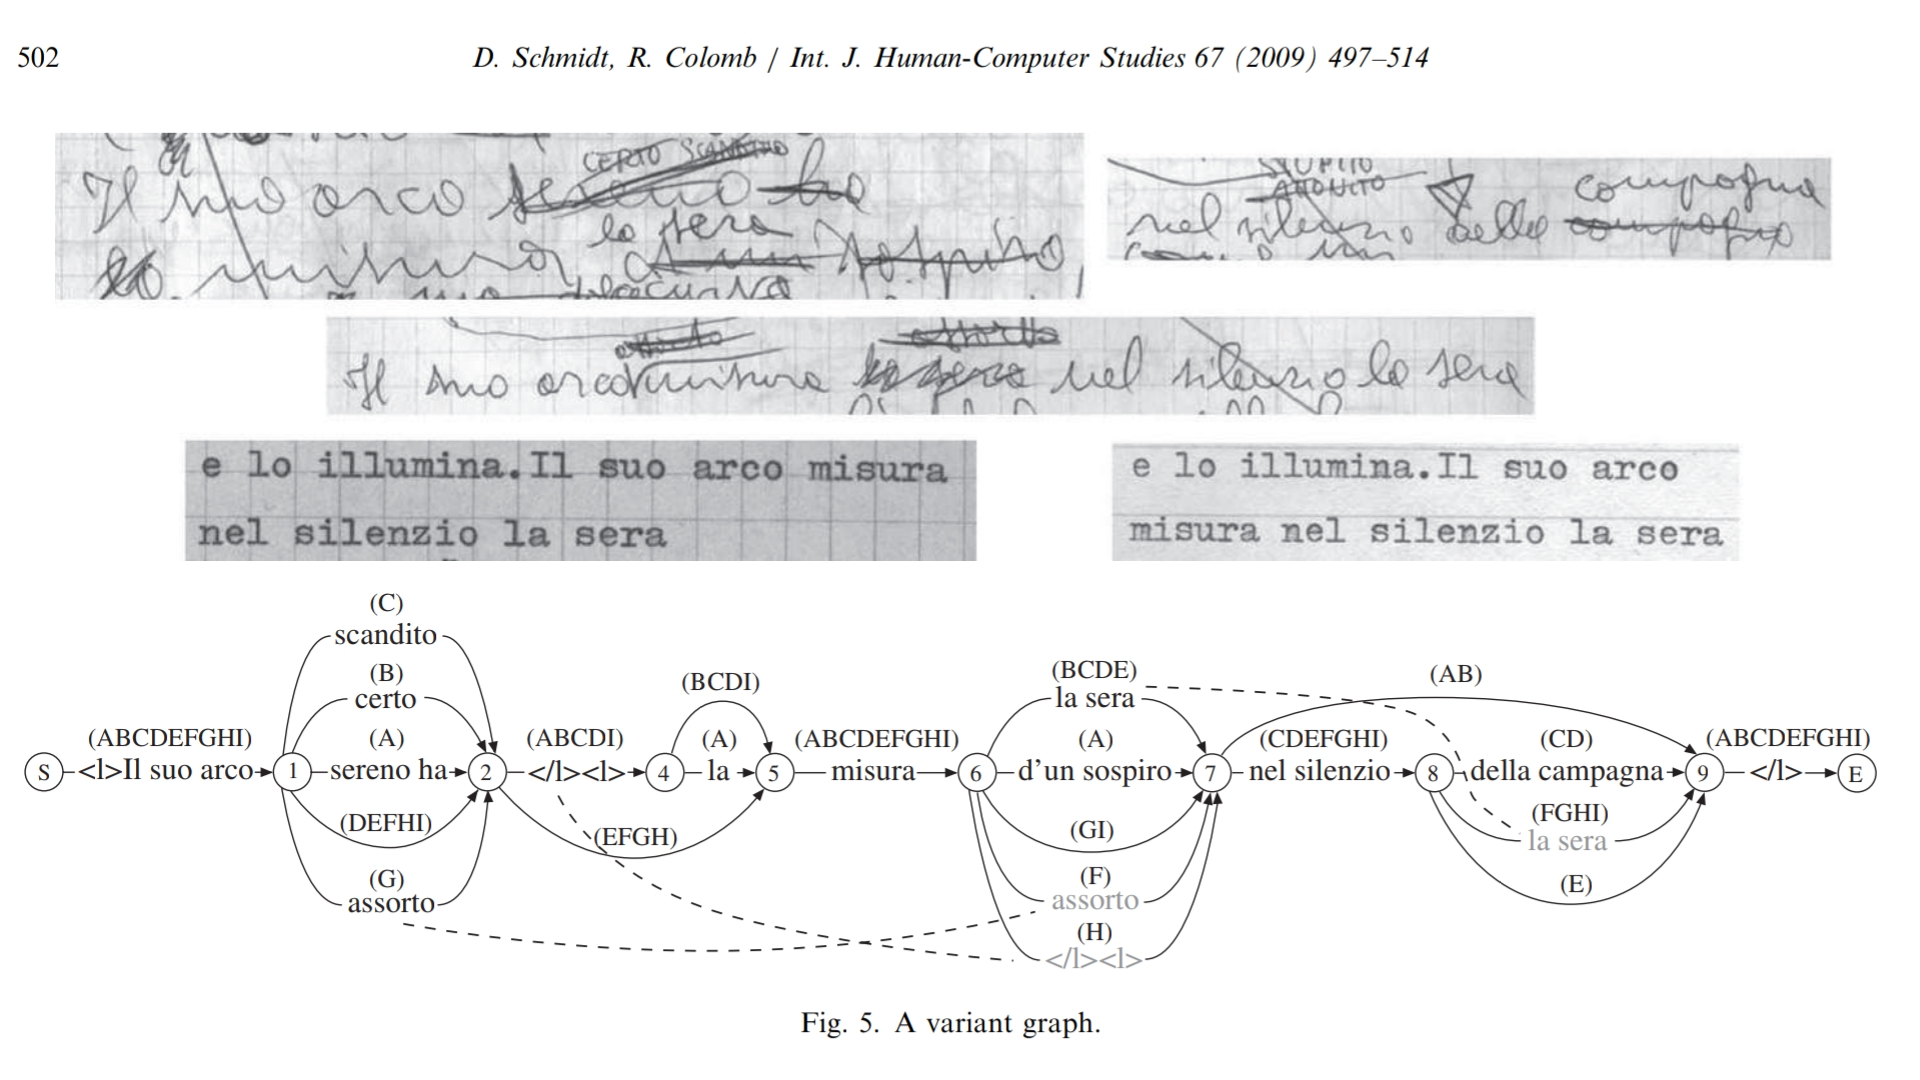
\includegraphics[scale=0.15]{text_variant_graph.jpg}
    \end{figure}
\end{frame}

\begin{frame}
    \frametitle{\emph{Variation graphs} project genomes into a graph}
%Textual ``variant graphs'' allow the compact description of a set of versions of a text.

    \begin{figure}
      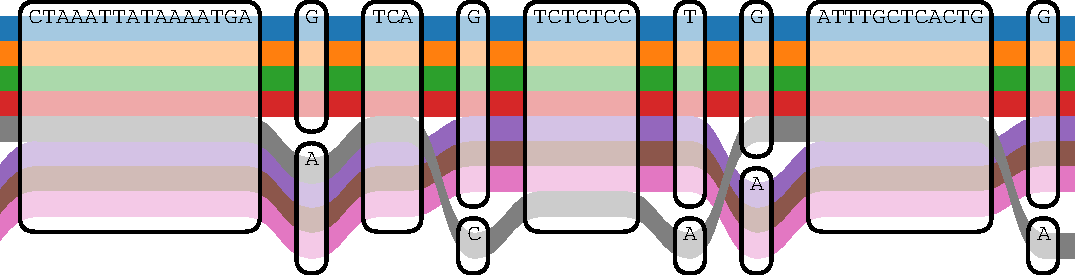
\includegraphics[scale=1.2,center]{vg_tubemap.pdf}
    \end{figure}
\end{frame}

\begin{frame}
  \frametitle{Whole genome alignments}
  \begin{columns}[c] % The "c" option specifies centered vertical alignment while the "t" option is used for top vertical alignment

    \column{.45\textwidth} % Right column and width
    Alignments of whole genomes are equivalently represented as a graph.
    \\~\\
    Here, the variation graph induced by \textsc{seqwish} from the  \textsc{minimap2} alignments of seven \emph{S. cerevisiae} genomes.
    \\~\\
    10.1038/ng.3847
    \column{.5\textwidth} % Left column and width

    \begin{figure}
      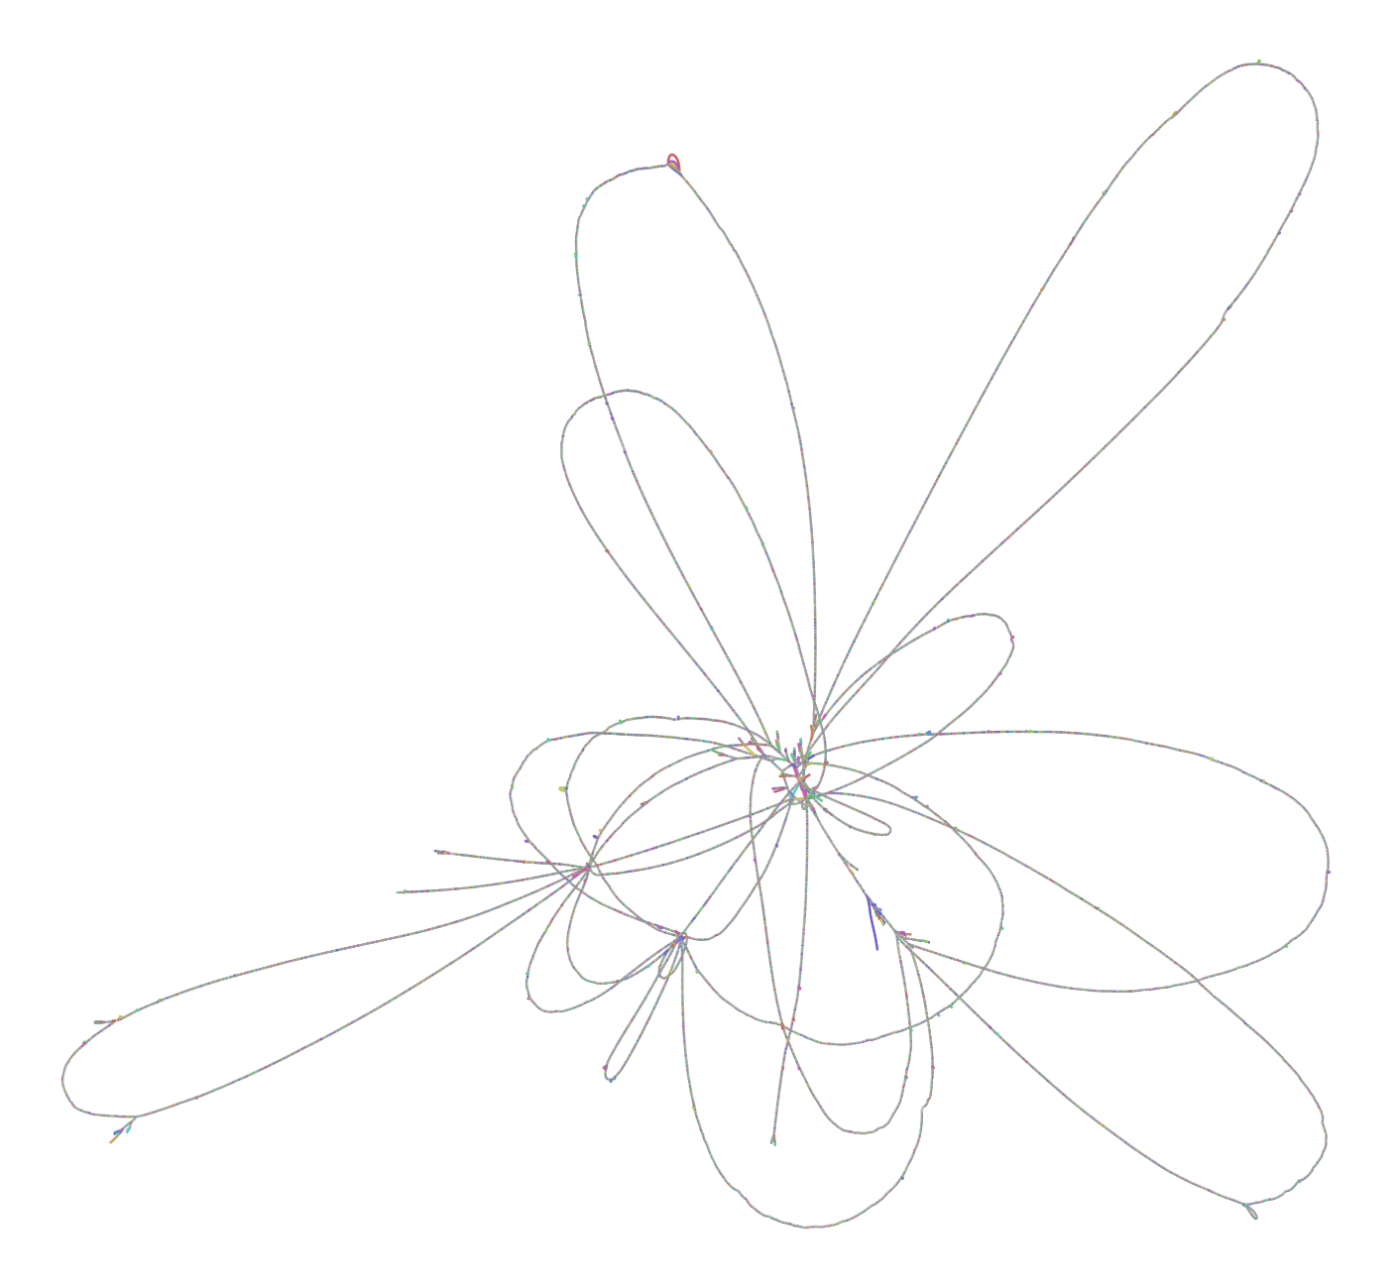
\includegraphics[scale=0.145,center]{seqwish_yeast.png}
    \end{figure}
  \end{columns}
\end{frame}


\subsection{Definitions}

\begin{frame}
  \begin{figure}
    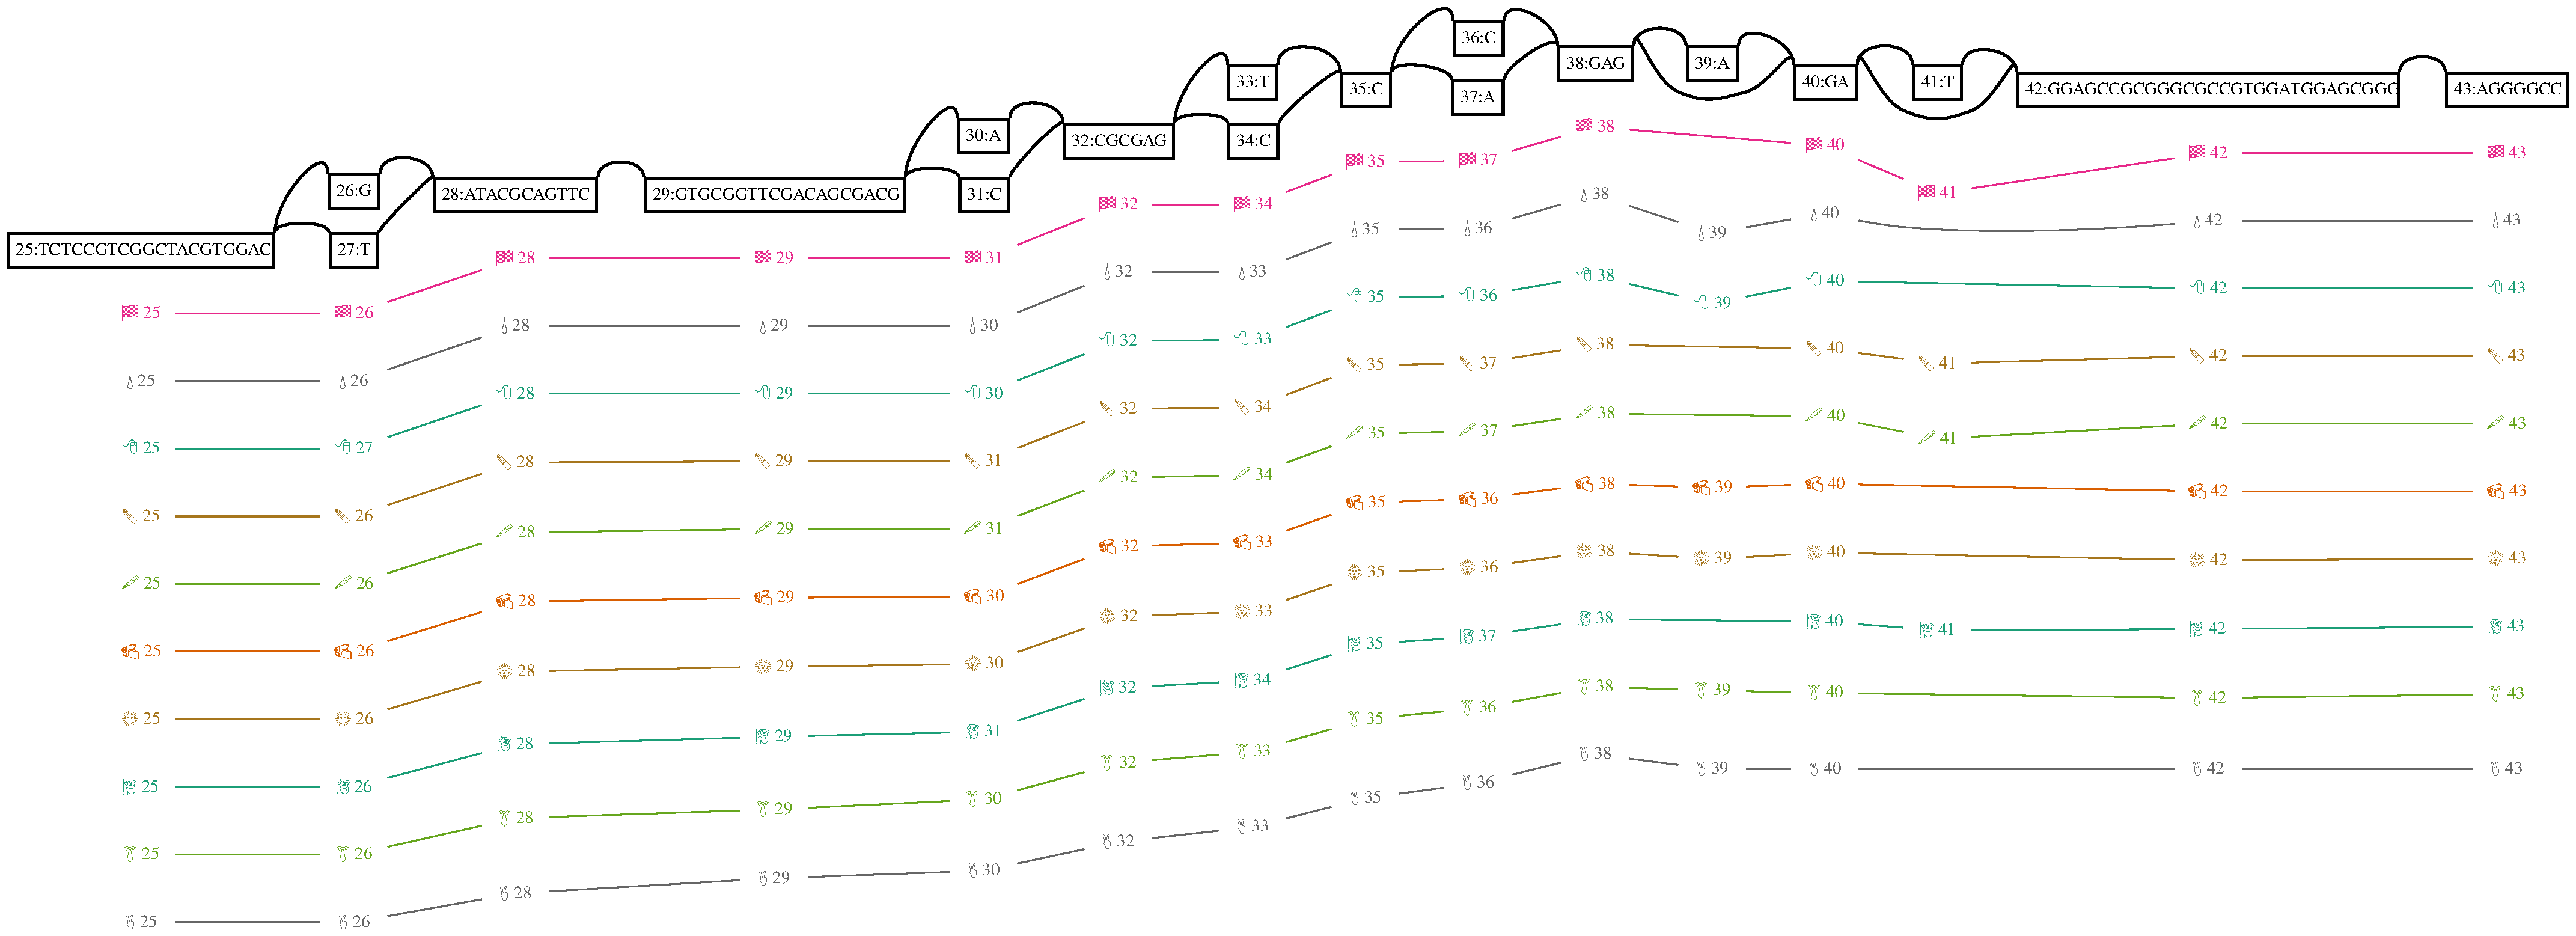
\includegraphics[scale=0.3,center]{H_3136.pdf}
  \end{figure}
\end{frame}

\begin{frame}
  \frametitle{The variation graph model}
  A \emph{variation graph} is a graph with paths: $G = (N, E, P)$.
\\~\\  
  \emph{nodes}: $N = n_1 \ldots n_{|N|}$
  
  \emph{edges}: $E = e_1 \ldots e_{|E|}$

  \emph{paths}: $P = p_1 \ldots p_{|P|}$
  \\~\\
  %Nodes of the graph are labeled with text, and so the nodes and edges can be thought of as a regular language model.
  The graph represents a collection of sequences, with each $p_i$ describing one embedding of a particular sequence within the graph.
  \\~\\
  To model DNA, the graph must be bidirectional and represent both strands of the molecule.
\end{frame}

\begin{frame}
  \frametitle{Nodes are labeled with sequences}
  Each node $n_i$ represents a sequence $seq(n_i)$ that is built from an alphabet $\Sigma = \{ {\tt A, C, G, T, N} \}$.
  \\~\\
  Nodes may be traversed in either the forward or reverse direction, with the sequence being reverse-complemented in the reverse direction.
  \\~\\
  We write $\overline{n_i}$ for the reverse-complement of node $n_i$, so that $seq(n_i) = revcomp(seq(\overline{n_i}))$.
  \\~\\
  Note that $n_i = \overline{\overline{n}}$. For convenience, we refer to both $n_i$ and $\overline{n_i}$ as ``nodes''.
\end{frame}

\begin{frame}
  \frametitle{Edges define allowed paths}
  Edges represent adjacencies between the sequences of the nodes they connect.
  \\~\\
  Thus, the graph implicitly encodes longer sequences as the concatenation of node sequences along walks through the graph.
  \\~\\
  Edges can be identified with the ordered pairs of oriented nodes that they link, so we can write $e_{ij} = (n_i,n_j)$.
  \\~\\
  Edges also can be traversed in either the forward or the reverse direction, with the reverse traversal defined as $\overline{e_{ij}} = (\overline{n_j},\overline{n_i})$.
%  \\~\\
%  VGs can contain ordinary cycles (in which $n_i$ is reachable from $n_i$), reversing cycles (in which $n_i$ is reachable from $\overline{n_i}$), and non-cyclic instances of reversal (in which both $n_i$ and $\overline{n_i}$ are reachable from $n_j$).
  %\\~\\
\end{frame}

%\subsection{Paths are essential}
\begin{frame}
  \frametitle{Paths make the $G$ lossless wrt. sequences}
  If $G = (N, E)$, the graph would do no better than a Markov model at simulating genomes.
  Natural sequences tend to have high long-range mutual information.
%  \\~\\
  \begin{figure}
    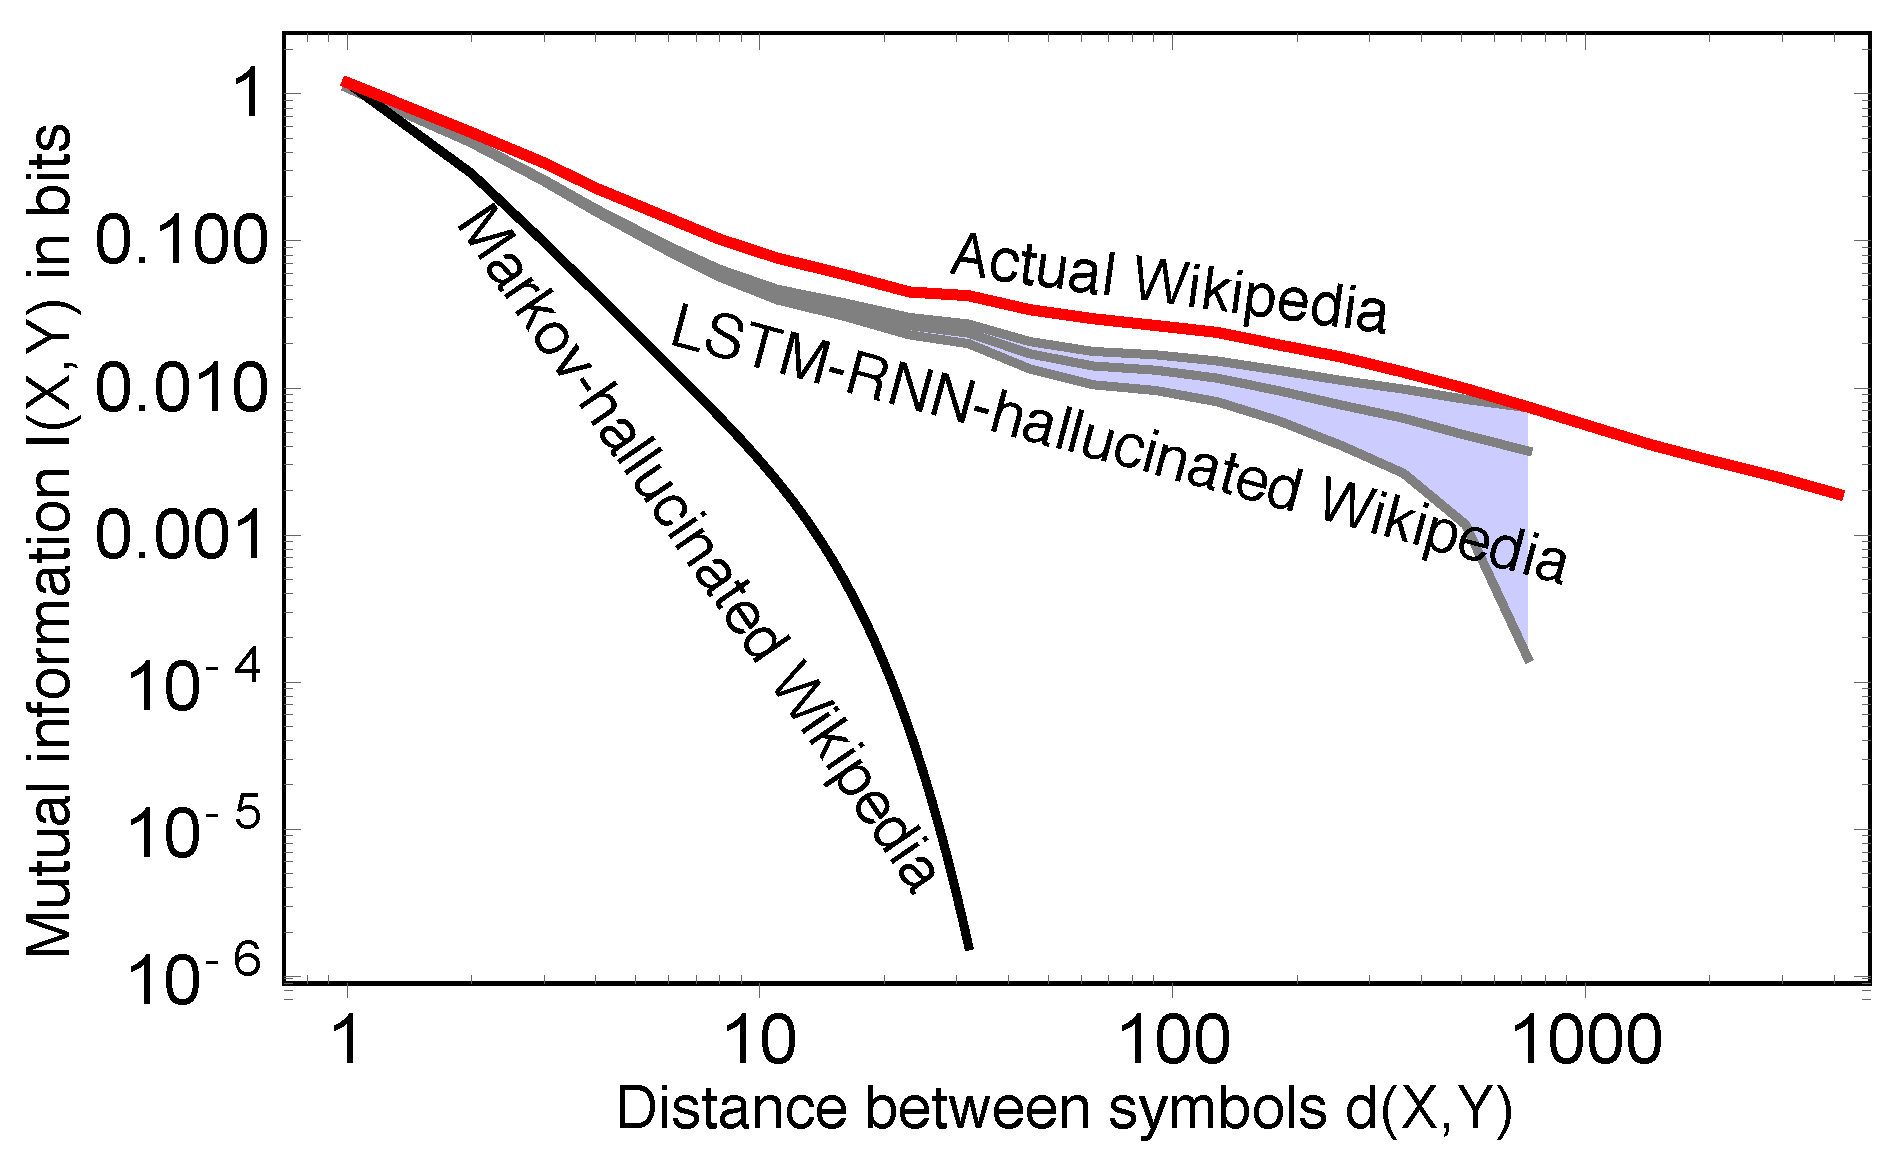
\includegraphics[scale=1,center]{entropy-19-00299-g003.png}
  \end{figure}

  \begin{flushright}
  \tiny{Entropy 2017, 19(7), 299; doi:10.3390/e19070299}
    \end{flushright}
\end{frame}

\section{Representing VGs}

\begin{frame}
  \frametitle{The variation graph toolkit: \textsc{vg}}
    We have implemented variation graph utilities in \textsc{vg}\footnote{\url{https://github.com/vgteam/vg}}.
  \begin{figure}
    
\includegraphics[scale=0.2,center]{vg_logo.png}
  \end{figure}
\end{frame}

\subsection{Handle graphs}
\begin{frame}[fragile]
  \frametitle{Handle graph interface}
  After working with variation graphs for some time, the \textsc{vgteam} has established a standard virtual API that graph backing implementations can match.
  \\~\\
  Opaque \emph{handles} that internally represent nodes and path steps are exposed directly to external algorithms without requiring indirection.
  \\~\\
  %64-bit handles are provided for nodes, where $n_i$ and $\overline{n_i}$ are distinct and the handle records the relative orientation.
  %\\~\\
  %Path steps are exposed as 128-bit records, and could represent e.g. node/path/rank for each path step.
%\end{frame}
%\begin{frame}[fragile]
  \begin{lstlisting}
    class HandleGraph { };
    class PathHandleGraph : virtual public HandleGraph { ... };
    class MutableHandleGraph : virtual public HandleGraph { ... };
    class DeletableHandleGraph : virtual public MutableHandleGraph { ... };
    class MutablePathHandleGraph : virtual public PathHandleGraph { ... };
    class MutablePathMutableHandleGraph :
        virtual public MutablePathHandleGraph,
        virtual public MutableHandleGraph { ... };
    class MutablePathDeletableHandleGraph :
        virtual public MutablePathHandleGraph,
        virtual public DeletableHandleGraph { ... };
  \end{lstlisting}
\end{frame}

\subsection{Dynamic, uncompressed}

\begin{frame}[fragile]
  \frametitle{\textsc{vg}'s dynamic graph}
  Represented naïvely, the dynamic graph implemented in \textsc{vg} consumes a lot of memory in hash tables and linked lists.
%  In \textsc{vg} we use hash tables to store node/edge/path relationships and linked lists to represent paths.
  \\~\\
  For the graph's nodes $N$:
  \begin{lstlisting}
    hash_map<id_t, Node*> node_by_id;
    hash_map<Node*, int> node_index;
  \end{lstlisting}
  ... its edges $E$:
  \begin{lstlisting}
    pair_hash_map<pair<NodeSide, NodeSide>, Edge*> edge_by_sides;
    hash_map<Edge*, int> edge_index;
    hash_map<id_t, vector<pair<id_t, bool>>> edges_on_start;
    hash_map<id_t, vector<pair<id_t, bool>>> edges_on_end;
  \end{lstlisting}
  and for each path $p_i \in P$:
  \begin{lstlisting}
    hash_map<const mapping_t*, pair<list<mapping_t>::iterator, int64_t> > mapping_itr;
    map<string, hash_map<size_t, mapping_t*>> mappings_by_rank;
    hash_map<id_t, map<int64_t, set<mapping_t*>>> node_mapping;
    set<id_t> head_tail_nodes;
  \end{lstlisting}
\end{frame}

\begin{frame}
  \frametitle{Memory woes}
  Loading a variation graph into memory with \textsc{vg}'s default dynamic model can require more than twenty times the uncompressed size in GFA\footnote{\url{https://github.com/GFA-spec/GFA-spec}}.
  \\~\\
  For the human genome and 1000 Genomes Project (1000GP) variation, where the GFA requires 20GB, loading the whole graph is expected to take around 400GB of memory\footnote{I actually haven't ever done this, because my testing is only on systems with $<$256GB of RAM.}.
  \\~\\
  Dynamic modification of the graph requires us partitioning the graph by chromosome, which is not tenable for large assembly graphs or in genome graphs with a lot of structural variation.
\end{frame}

\subsection{Static, succinct}
\begin{frame}[fragile]
  \frametitle{Compact static variation graph}
  To hold large graphs in memory during DNA sequence read alignments, we developed the \textsc{xg} succinct variation graph.
  \\~\\
  The basic idea is to compact the graph into a set of succinct data structures that provide decent cache locality when traversing the graph.
  \\~\\
  This self index is capable of storing the 1000GP graph in 30GB.
  \\~\\
  To build it we don't use the \textsc{vg} class, but a lighter-weight hash based graph model, which still requires $>$100GB of RAM!
  \\~\\
  It supports graph topology, node sequence, path membership, and path position queries.
\end{frame}

\begin{frame}
  \frametitle{\textsc{xg} index of $G = (N, E, P)$}
  The graph is stored in vector $G_\mathbf{iv} = g_1 \ldots g_{|N|}$, with $g_i = ( \eta_i, \Xi_i)$
  \\~\\
  $\eta_i = \left[ id(i), seq_\mathbf{offset}(n_i), |seq(n_i)|, in(n_i), out(n_i) \right]$.
  \\~\\
  $\Xi_i$ is a packed, relativistic recording of the edge context of $n_i$.
  \\~\\
  Bitcompressed vector $S_\mathbf{iv}$ stores the sequence labels of nodes.
  \\~\\
  Paths are recorded in mapping $N_\mathbf{path}$ and a set of per-path vectors that allow for positional and topological queries.
  \\~\\
  Bitvectors featuring $rank(i,c)$ and $select(i,c)$ allow us to map between node ids and these structures.
\end{frame}

\begin{frame}
  \frametitle{\textsc{xg} sketch}
  \begin{figure}
    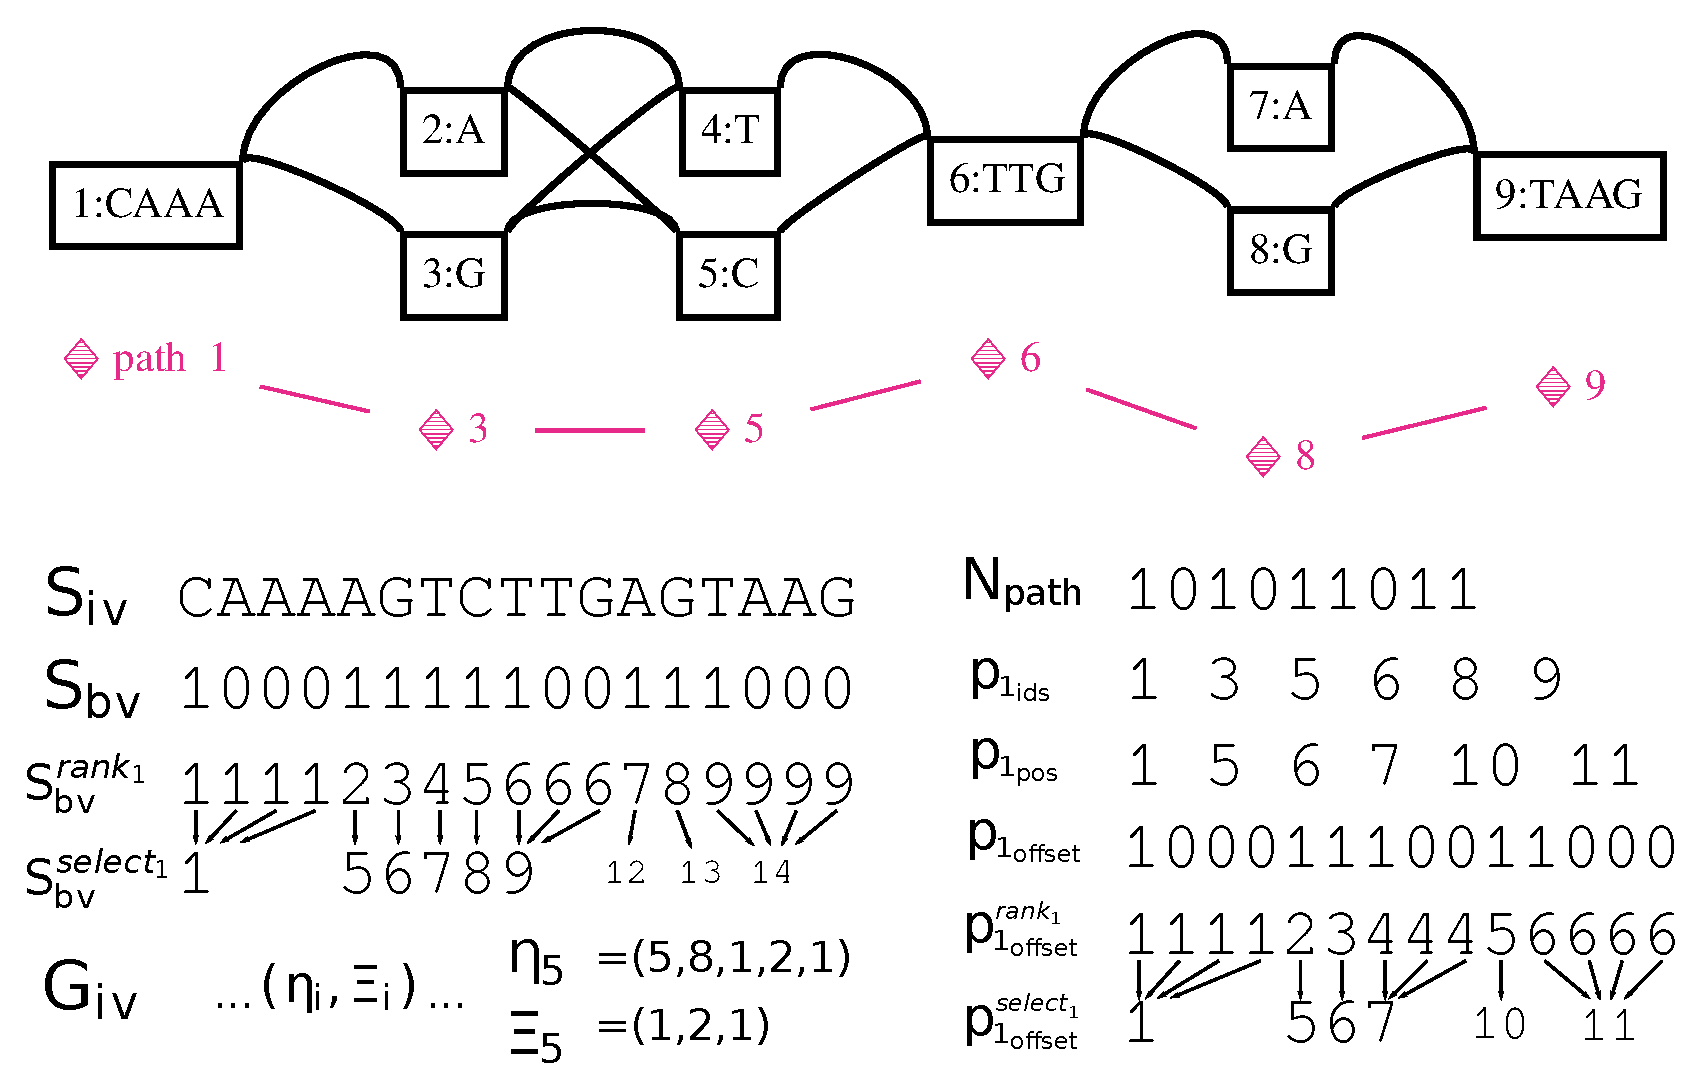
\includegraphics[scale=0.375,center]{xg_index_sketch_nice.pdf}
  \end{figure}
\end{frame}

\begin{frame}
  \frametitle{The Graph Burrows Wheeler Transform}
  Sirén's GBWT (and the related gPBWT) use the BWT of haplotypes through the graph to build a compact index of paths.

  \begin{figure}
    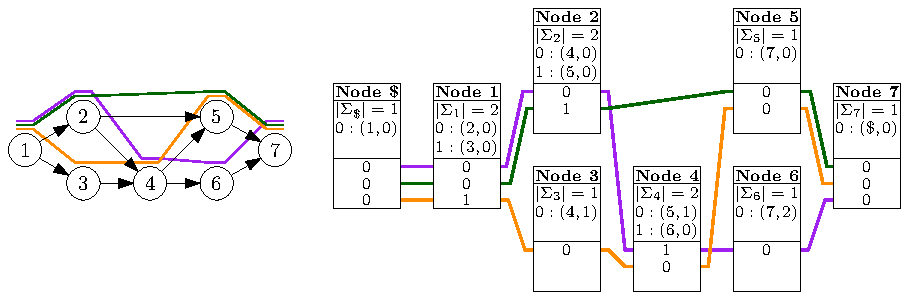
\includegraphics[scale=0.75,center]{gbwt-example.pdf}
  \end{figure}

  The repetitive nature of the paths generated by real genomes makes the GBWT very compressible.
  The GBWT allows for efficient $O(|p|)$ haplotype matching.
\end{frame}

\subsection{Dynamic, succinct}

\begin{frame}[fragile]
  \frametitle{``dank'' graphs: \textsc{dsgvg}}
  The ideal VG would be fully dynamic, but small and efficient.
  \\~\\
  To implement such a graph, we have extended DYNAMIC\footnote{\url{https://github.com/vgteam/DYNAMIC}} to provide dynamic locally-packed integer vectors based on a B+-tree, and otherwise used standard structures provided by the library. These provide rank, select, insert, and remove.
  \\~\\
  \begin{columns}[c] % The "c" option specifies centered vertical alignment while the "t" option is used for top vertical alignment

    \column{.5\textwidth} % Right column and width
    Nodes and edges:
    \begin{lstlisting}
      lciv_iv graph_id_iv;
      suc_bv deleted_id_bv;
      hash_map<uint64_t, uint64_t> graph_id_map;
      hash_set<uint64_t> graph_id_hidden_set;
      lciv_iv topology_iv;
      suc_bv topology_bv;
    \end{lstlisting}

    \column{.5\textwidth} % Left column and width
    Paths:
    \begin{lstlisting}
      dyn::packed_vector seq_pv;
      suc_bv seq_bv;
      wt_str path_handle_wt;
      lciv_iv path_rev_iv;
      lciv_iv path_next_id_iv;
      lciv_iv path_next_rank_iv;
      lciv_iv path_prev_id_iv;
      lciv_iv path_prev_rank_iv;
    \end{lstlisting}
  \end{columns}
\end{frame}

\begin{frame}
  \frametitle{\textsc{dsgvg} summary}
  As in GBWT, we can exploit the typical structure of variation graphs (linear, with some structural variants and long-range joins) to reduce the local alphabet size.
  \\~\\
  We relativistically encode edges $e_{ij}$ as $i - j$.
  \\~\\
  Paths are also relativistically encoded.
  Each entry in the path vectors refers to a path step on a particular node.
  We record the next and previous steps to allow path traversal.
  Path records are recorded as $node(p_i) - node(p_j)$, and as the rank of the particular path on that node, which allows for cycles.
\end{frame}

\begin{frame}[fragile]
  \frametitle{\textsc{dsgvg} sketch}
      {\tiny
\begin{verbatim}
graph_id_map 5->4 7->6 8->7 1->0 4->3 6->5 2->1 9->8 3->2 
graph_id_iv	 1 2 3 4 5 6 7 8 9 0 
del_id_bv    0 0 0 0 0 0 0 0 0 1
topology_iv  2 4 0 2 0 3 6 0 4 0 3 4 3 4 0 2 0 5 4 3 4 0 3 4 5 4 3 2 0 5 4 7 4 4 4 0 2 0 3 4 5 4 2 4 0 3 4 2 2 0 5 4 2 3 4 5 4
topology_bv  1 0 0 0 0 1 0 0 0 0 0 0 1 0 0 0 0 0 0 1 0 0 0 0 0 0 1 0 0 0 0 0 0 1 0 0 0 0 0 0 0 0 1 0 0 0 0 1 0 0 0 0 1 0 0 0 0 1
seq_pv       3 1 1 1 2 1 1 4 1 4 2 3 2 2 4 1 4 1 1 1 2 2 2 2 3 2 
seq_bv       1 0 0 0 0 0 0 0 1 1 1 1 1 0 0 1 1 1 0 0 0 0 0 0 0 0 1
p_handle_wt  0 1 0 0 1 0 0 1 0 1 0 0 1 0 1 0 
p_rev_iv     0 0 0 0 0 0 0 0 0 0 0 0 0 0 0 0 
p_next_id_iv 0 6 0 0 6 0 0 4 0 6 0 0 4 0 $ 0 
p_next_rn_wt 0 0 0 0 0 0 0 0 0 0 0 0 0 0 0 0 
p_prev_id_iv 0 ^ 0 0 7 0 0 7 0 5 0 0 7 0 5 0 
p_prev_rn_wt 0 0 0 0 0 0 0 0 0 0 0 0 0 0 0 0 
p_metadata   0:x:0/0->8/0 
\end{verbatim}
      }
        \begin{figure}
    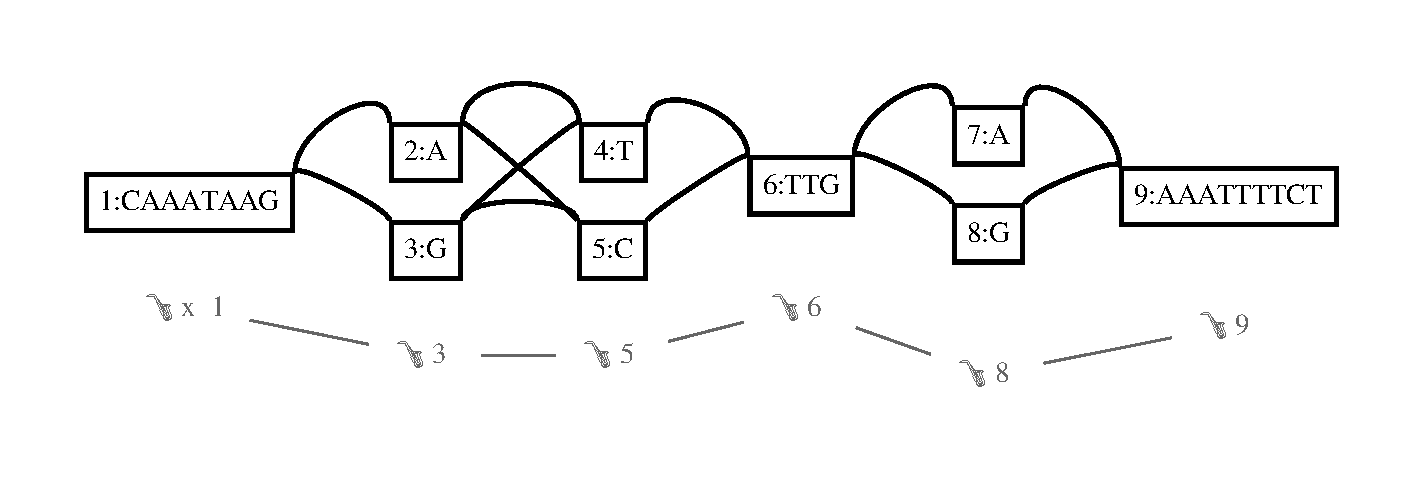
\includegraphics[scale=0.4,center]{w_graph.pdf}
  \end{figure}

\end{frame}

\begin{frame}
  \frametitle{A note on wavelet trees and wavelet matrixes}
  \begin{figure}
    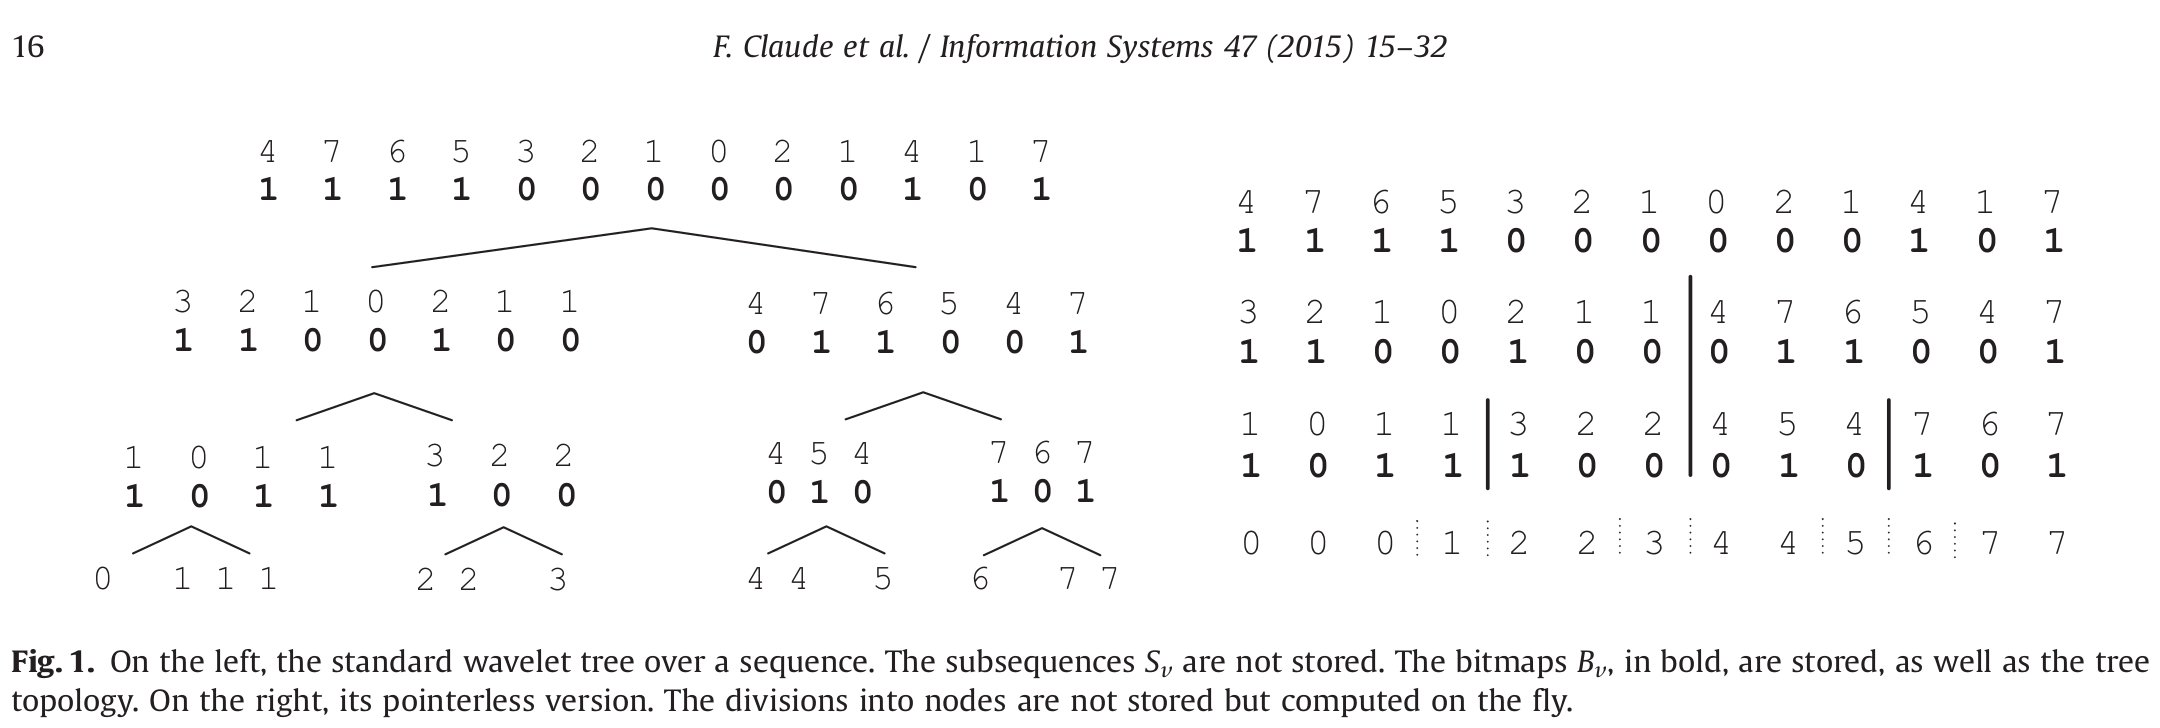
\includegraphics[scale=0.12,center]{wt_ptr_and_non.png}
  \end{figure}
  \begin{figure}
    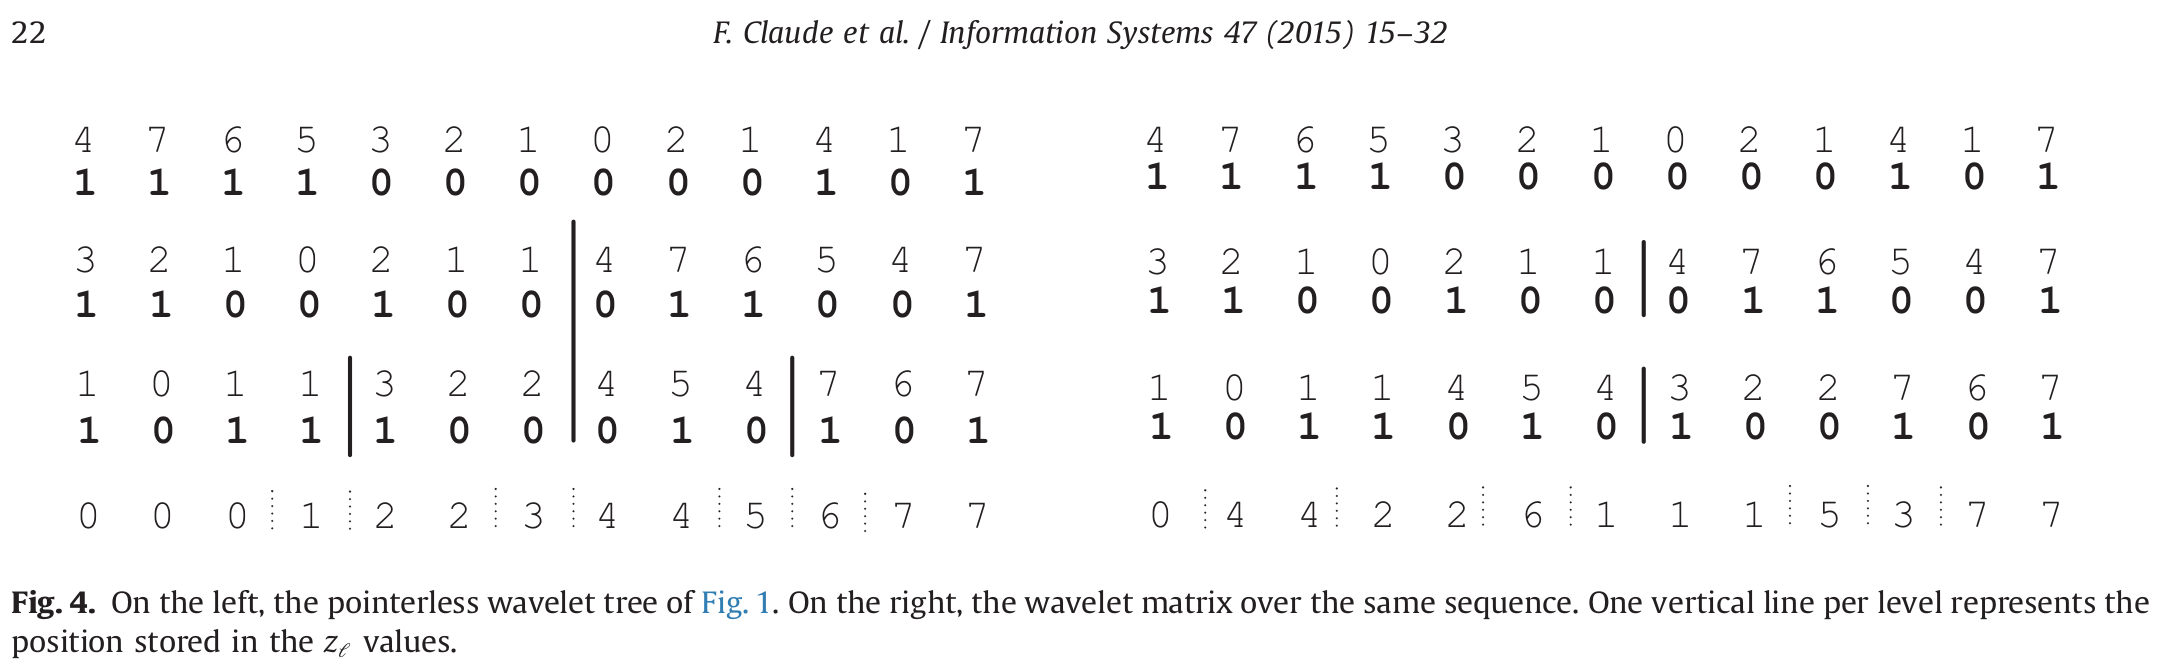
\includegraphics[scale=0.12,center]{wt_ptr_and_wm.png}
  \end{figure}
\end{frame}

\begin{frame}
  \frametitle{A note on wavelet trees and wavelet matrixes}
  The DSGVG could be implemented more compactly using a wavelet matrix.
  This would avoid the high cost of alphabet size when using a pointer based wavelet tree.
  \\~\\
  \begin{itemize}
  \item One WM could store the node id to handle rank mapping, avoiding the need for a deletion state vector and garbage collection.
  \item The graph topology could be stored non-relativistically in a WM, providing simpler queries.
  \item A WM built from concatenated paths $\$p_1\$p_2\$\ldots\$p_{|P|}\$$ would support path$\to$node and node$\to$path mapping, and simple updates of paths without auxiliary structures.
  \end{itemize}
\end{frame}

\begin{frame}
  \frametitle{No dynamic wavelet matrix implementation exists}
  In ``Practical Dynamic Entropy-Compressed Bitvectors with Applications'' (10.1007/978-3-319-38851-9\_8, 2016), the authors provide a URL for their implementation, but the code was never posted.
  \\~\\
  This would be really useful, but in the interest of time I have not pursued a new implementation of it.
\end{frame}

\section{Results}

\subsection{Graphs from the 1000GP}

\begin{frame}
  \frametitle{1000GP graphs}
  These graphs are built from the variant list in the 1000GP. They contain only the reference path, and have dense variation (one variant every 11bp).
  \begin{center}
  \begin{tabular}{ | c | c | c | c | c | c | }
    \hline
    graph & GFA & XG & DSGVG & \textsc{vg} stats & \textsc{dsgvg} stats \\
    \hline
    \hline
    1Mbp & 5.3MB & 9.7MB & 3.8M & 0.64s & 0.21s \\
    chr20 & 438MB & 620MB & 249MB & 64.8s & 20.5s \\
    chr8 & 1.1GB & 1.6GB & 610MB & 175s & 50.5s \\
    chr2 & 1.6GB & 2.4GB & 968MB & 291s & 82.6s \\
    1000GP & 20GB & 30GB & 12GB & n/a & 1265s \\
    \hline  
  \end{tabular}
  \end{center}
\end{frame}

\subsection{\emph{S. cerevisiae} graphs}

\begin{frame}[fragile]
  \frametitle{\emph{S. cerevisiae} whole genome alignment graphs}
  \begin{columns}[c] % The "c" option specifies centered vertical alignment while the "t" option is used for top vertical alignment
    \column{.5\textwidth} % Right column and width
    \textsc{Cactus} graph %(LASTZ$\to$\textsc{Cactus}$\to$GFA)
    \begin{figure}
      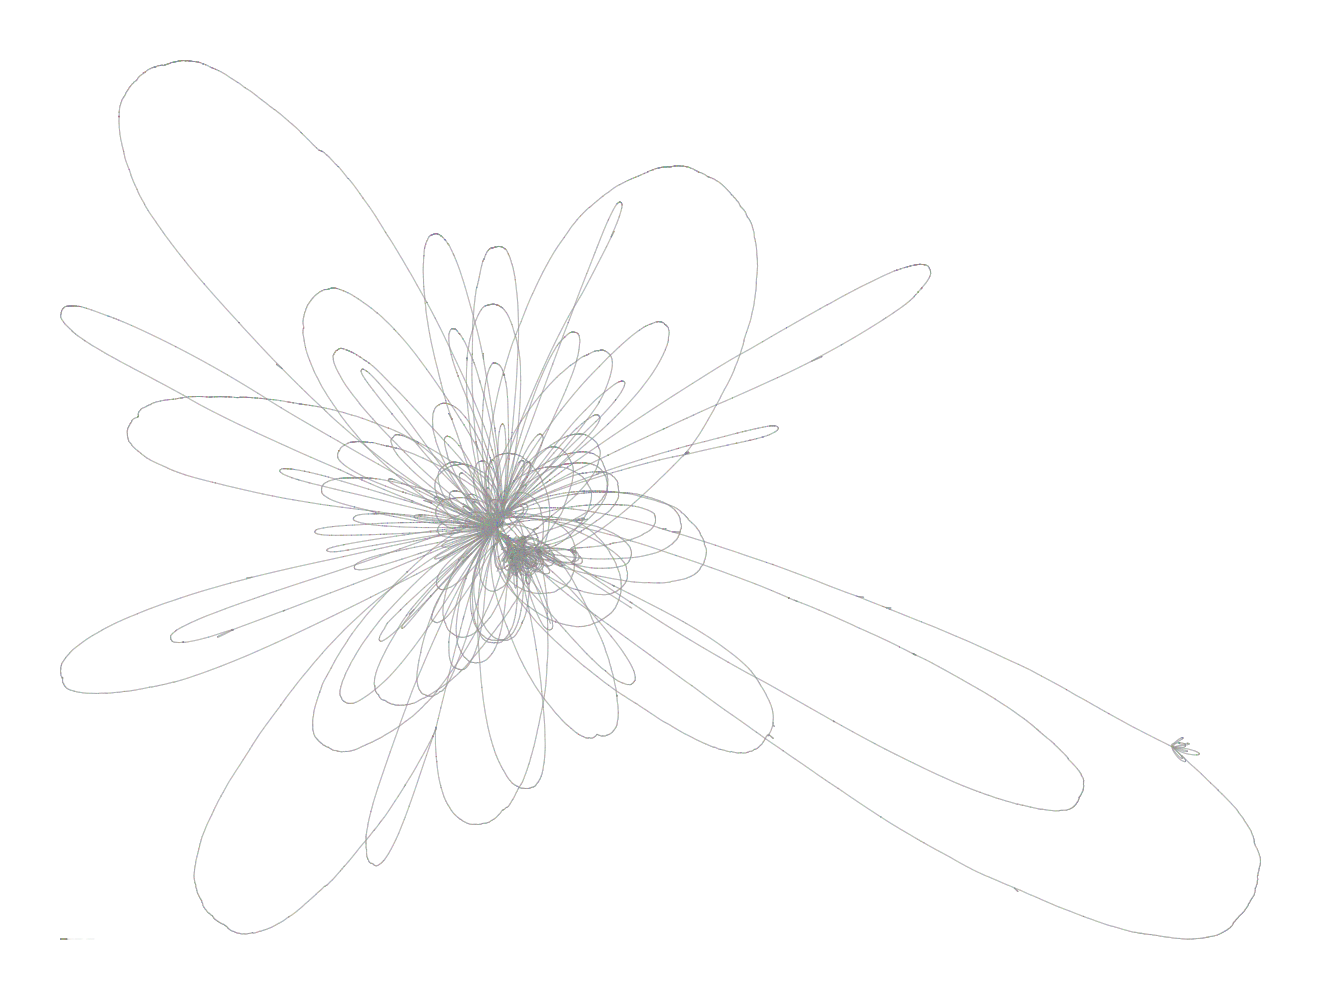
\includegraphics[scale=0.18,center]{cactus_yeast.png}
    \end{figure}
    \column{.5\textwidth} % Left column and width
    \textsc{seqwish} graph %(\textsc{minimap2}$\to$\textsc{seqwish}$\to$GFA)
    \begin{figure}
      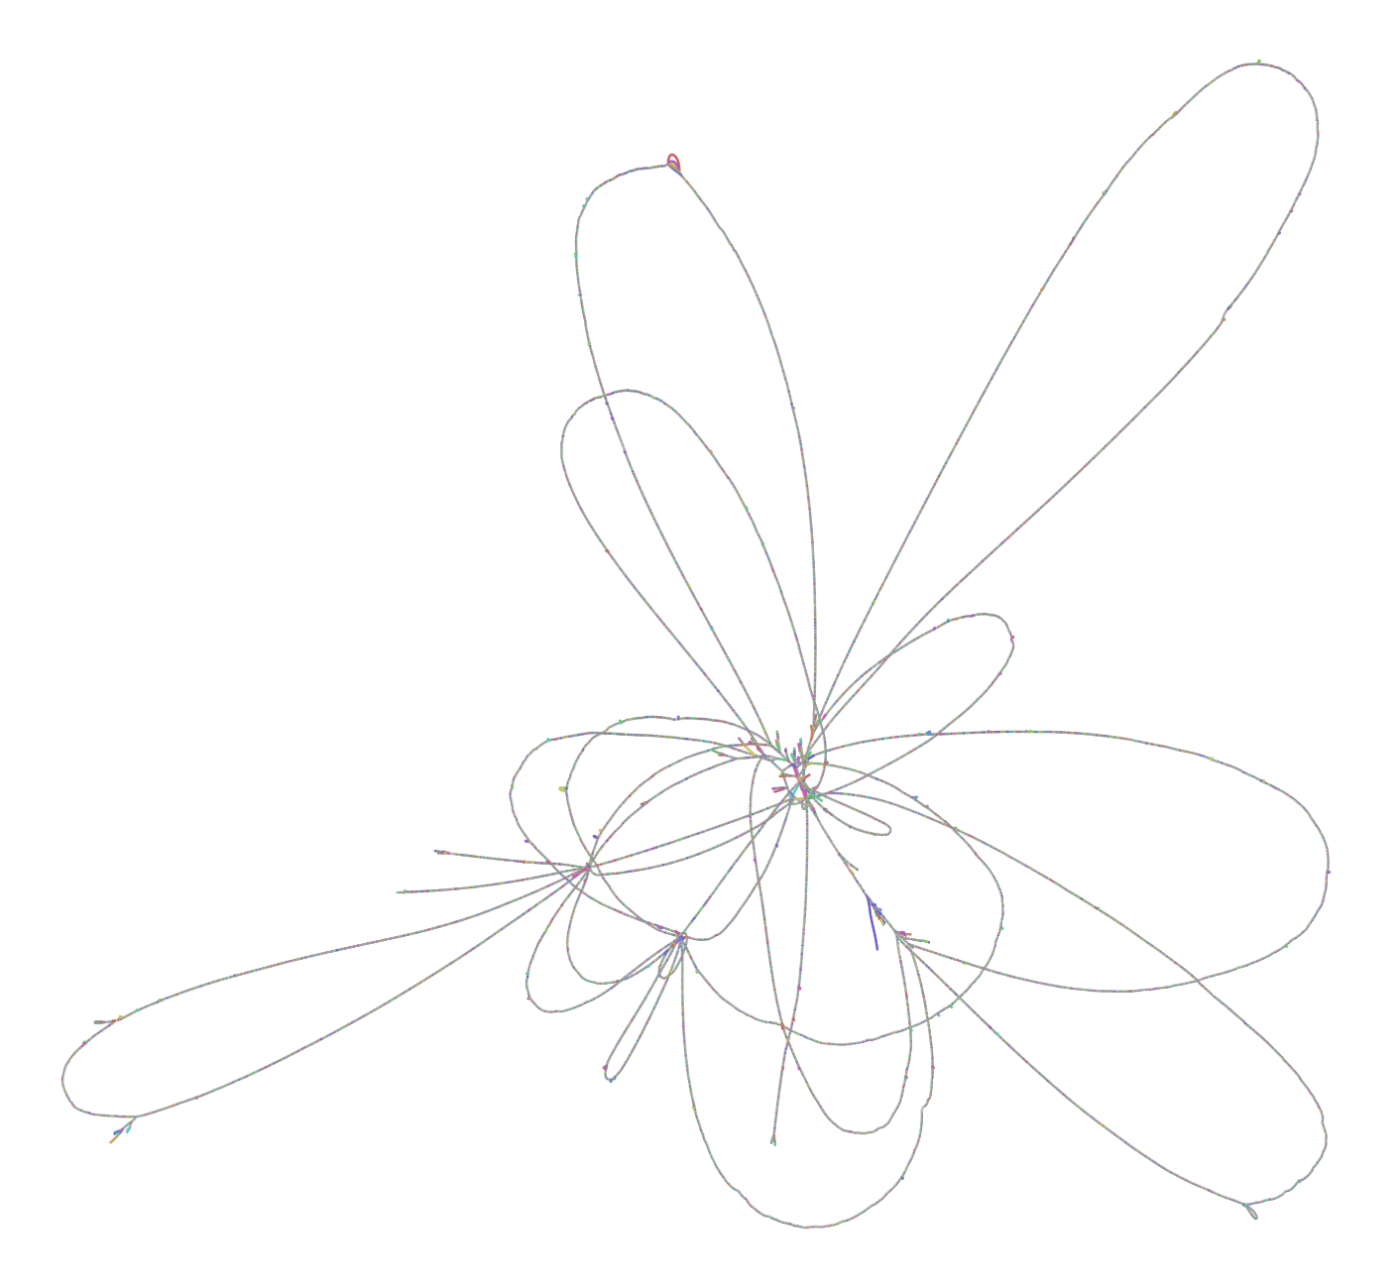
\includegraphics[scale=0.10,center]{seqwish_yeast.png}
    \end{figure}
  \end{columns}
    \begin{center}
  \begin{tabular}{ | c | c | c | c | c | c | }
    \hline
    graph & GFA & XG & DSGVG & \textsc{vg} stats & \textsc{dsgvg} stats \\
    \hline
    \hline
    cactus & 115MB & 66MB & 81MB & 34.8s & 2.31s \\
    seqwish & 92MB & 44MB & 77MB & 18.6s & 1.50s \\
    \hline  
  \end{tabular}
  \end{center}
\end{frame}

\subsection{Larger whole genome alignments}
\begin{frame}
  \frametitle{A cichlid pangenome}
  Alignment of four cichlid (and related) genomes.
  Each genome is around 1GBp, and the GFA produced by \textsc{seqwish} is 14GB.
  The resulting \textsc{dsgvg} index is 11GB.
  It was impossible to process this graph with \textsc{vg}.
  \begin{figure}
    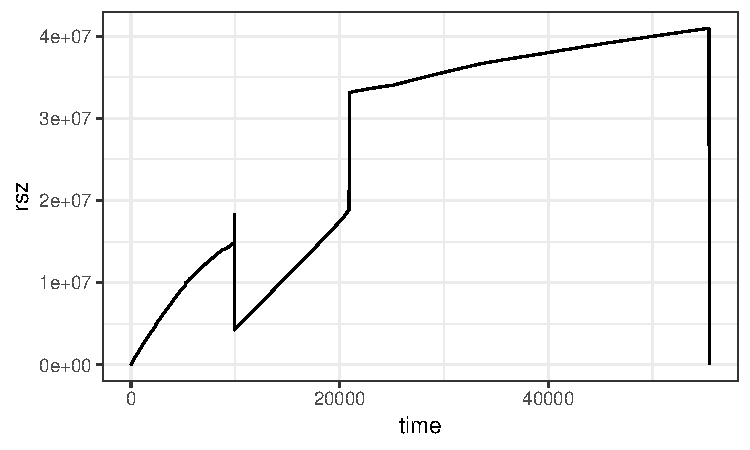
\includegraphics[scale=0.7,center]{cichlid_log.pdf}
  \end{figure}
\end{frame}

\subsection{Testing}
\begin{frame}
  \frametitle{Unit tests}
  Although I'm not providing numbers, the graph is in fact dynamic and it's tested. See \url{https://github.com/vgteam/dsgvg}
\end{frame}

\section{Conclusions}
\begin{frame}
  \frametitle{Conclusions!}
  We have implemented a dynamic succinct genome variation graph model.
  Next steps...
\end{frame}

\end{document} 
